\documentclass[11pt]{article}

\usepackage{filecontents}
\begin{filecontents}{\jobname.bib}
@article{hohna2014probabilistic,
  title={Probabilistic graphical model representation in phylogenetics},
  author={H{\"o}hna, Sebastian and Heath, Tracy A and Boussau, Bastien and Landis, Michael J and Ronquist, Fredrik and Huelsenbeck, John P},
  journal={Systematic biology},
  volume={63},
  number={5},
  pages={753--771},
  year={2014},
  publisher={Oxford University Press}
}
@article{leliaert2014dna,
  title={DNA-based species delimitation in algae},
  author={Leliaert, Frederik and Verbruggen, Heroen and Vanormelingen, Pieter and Steen, Frederique and L{\'o}pez-Bautista, Juan M and Zuccarello, Giuseppe C and De Clerck, Olivier},
  journal={European journal of phycology},
  volume={49},
  number={2},
  pages={179--196},
  year={2014},
  publisher={Taylor \& Francis}
}
@article{ree2008maximum,
  title={Maximum likelihood inference of geographic range evolution by dispersal, local extinction, and cladogenesis},
  author={Ree, Richard H and Smith, Stephen A},
  journal={Systematic Biology},
  volume={57},
  number={1},
  pages={4--14},
  year={2008},
  publisher={Oxford University Press}
}
\end{filecontents}

\usepackage{natbib}
\usepackage{adjustbox}
\usepackage{amsmath}
\usepackage[font=footnotesize]{caption}
\usepackage[dvipsnames]{xcolor}
\usepackage{geometry}
  \geometry{margin=1in}
\usepackage{framed}
\usepackage[breaklinks]{hyperref}
\usepackage{minibox}
\usepackage[compact]{titlesec}
\usepackage{listings,color}

\definecolor{verbgray}{gray}{0.9}

\lstnewenvironment{code}{%
  \lstset{backgroundcolor=\color{verbgray},
  frame=single,
  framerule=0pt,
  basicstyle=\ttfamily\scriptsize,
  columns=fullflexible}}{}

\definecolor{shadecolor}{rgb}{.9, .9, .9}

\graphicspath{ {./figures/} }




\begin{document}


\noindent
\large
\begin{minipage}{0.5\textwidth}
\begin{flushleft} 
IB200, Spring 2016
\end{flushleft}
\end{minipage}
\begin{minipage}{0.5\textwidth}
\begin{flushright} 
\textit{University of California, Berkeley}
\end{flushright}
\end{minipage}

\vspace{0.5cm}


\begin{center}
\Large \textbf{Lab 11:} \\
Probabilistic Models of \\
Geographic Range Evolution \\
\normalsize
\textit{By Will Freyman} \\
\end{center}

\vspace{0.5cm}

\section{Before you begin}

Today's lab will be completed in R.
Please install R: \url{https://www.r-project.org/}

We'll be using the excellent R package \textbf{BioGeoBears}
which was developed by Nick Matkze, who was a GSI of this course!
His website (and the source of the example script we'll use)
is here:
\url{http://phylo.wikidot.com/biogeobears}

\section{Introduction to probabilistic biogeography models}


Probabilistic modeling of geographic range evolution 
allows us to use the standard set of statistical model choice
procedures (e.g. AIC, BIC, likelihood ratios, etc.)
to test different biogeographical scenarios,
and to make statistically sound inference of ancestral
geographic ranges over a phylogeny.
For example, we can test whether the observed 
biogeographic distribution of a clade is best
explained with a model that allows for 
vicariance and long-distance dispersal versus
a model that allows for only vicariance.

There are many parsimony based approaches for
studying biogeography that will be covered in lecture.
The first likelihood approaches to biogeography
were presented in the ground breaking \citet{ree2008maximum}.
We'll discuss these probabilistic models and their many
extensions in lecture (also see Figure 1 for a summary),
so here we'll focus on applying them
to the the phylogeny of the Hawaiian members of the
plant genus \textit{Psychotria} published in
\citet{ree2008maximum}.



\begin{figure}
\centering
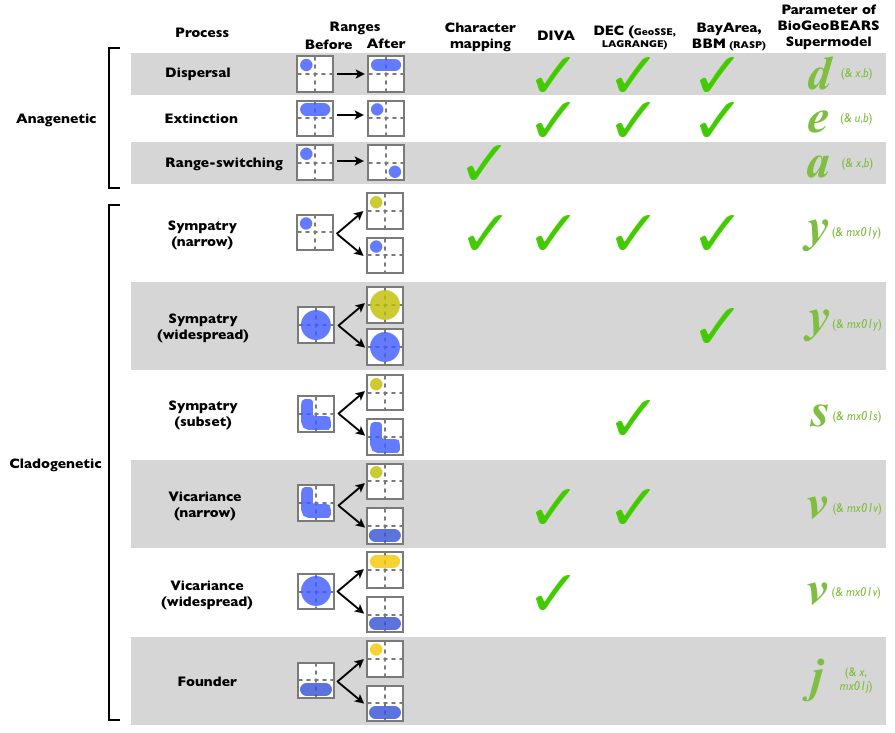
\includegraphics[width=0.9\textwidth]{BioGeoBEARS_supermodel.png}
\caption{
The processes assumed by different historical biogeography methods. Each of these processes is controlled by the specified parameter(s) in the BioGeoBEARS supermodel, allowing them to be turned on or off, or estimated from the data. Note that whether or not the data support a particular free parameter is an empirical question that should be tested with model choice procedures. Note also that this graphic deals only with the range-changing processes assumed by the different methods. BioGeoBEARS does not attempt to replicate e.g. the parsimony aspect of DIVA, just the processes allowed by DIVA (the BioGeoBEARS ``DIVA'' model could be called ``DIVALIKE'' to emphasize that it is a likelihood implementation of the processes assumed by DIVA).
Text and image from \protect\url{http://phylo.wikidot.com/biogeobears\#BioGeoBEARS\_supermodel\_graphic}.}
\end{figure}


\section{Installing BioGeoBears}

We will use BioGeoBears to implement the
2-parameter Dispersal-Extinction-Cladogeneis (DEC) 
model from \citet{ree2008maximum}
as well as the DEC+J model that includes
a long distance dispersal 
(jump or founder event speciation)
parameter.
See Figure 1 for details on the different models.
We'll use the Likelihood Ratio Test (LRT) and
Akaike information criterion (AIC)
to see which model fits the data better.

\subsection{Install and setup BioGeoBears}

Start up R and be sure to set your working directory so that you can
find the output file we will be generating (look back at
previous labs if you don't remember how to set the working directory). 
Install the BioGeoBears package:
\begin{code}
install.packages("BioGeoBEARS", dependencies=TRUE, repos="http://cran.rstudio.com")
\end{code}
Now lets load the package and some dependencies:
\begin{code}
library(optimx)
library(FD)
library(snow)
library(parallel)
library(BioGeoBEARS)
\end{code}
Now let's load some of the source files necessary to run BioGeoBears:
\begin{code}
source("http://phylo.wdfiles.com/local--files/biogeobears/cladoRcpp.R")
source("http://phylo.wdfiles.com/local--files/biogeobears/BioGeoBEARS_add_fossils_randomly_v1.R")
source("http://phylo.wdfiles.com/local--files/biogeobears/BioGeoBEARS_basics_v1.R")
source("http://phylo.wdfiles.com/local--files/biogeobears/BioGeoBEARS_calc_transition_matrices_v1.R")
source("http://phylo.wdfiles.com/local--files/biogeobears/BioGeoBEARS_classes_v1.R")
source("http://phylo.wdfiles.com/local--files/biogeobears/BioGeoBEARS_detection_v1.R")
source("http://phylo.wdfiles.com/local--files/biogeobears/BioGeoBEARS_DNA_cladogenesis_sim_v1.R")
source("http://phylo.wdfiles.com/local--files/biogeobears/BioGeoBEARS_extract_Qmat_COOmat_v1.R")
source("http://phylo.wdfiles.com/local--files/biogeobears/BioGeoBEARS_generics_v1.R")
source("http://phylo.wdfiles.com/local--files/biogeobears/BioGeoBEARS_models_v1.R")
source("http://phylo.wdfiles.com/local--files/biogeobears/BioGeoBEARS_on_multiple_trees_v1.R")
source("http://phylo.wdfiles.com/local--files/biogeobears/BioGeoBEARS_plots_v1.R")
source("http://phylo.wdfiles.com/local--files/biogeobears/BioGeoBEARS_readwrite_v1.R")
source("http://phylo.wdfiles.com/local--files/biogeobears/BioGeoBEARS_simulate_v1.R")
source("http://phylo.wdfiles.com/local--files/biogeobears/BioGeoBEARS_SSEsim_makePlots_v1.R")
source("http://phylo.wdfiles.com/local--files/biogeobears/BioGeoBEARS_SSEsim_v1.R")
source("http://phylo.wdfiles.com/local--files/biogeobears/BioGeoBEARS_stochastic_mapping_v1.R")
source("http://phylo.wdfiles.com/local--files/biogeobears/BioGeoBEARS_stratified_v1.R")
source("http://phylo.wdfiles.com/local--files/biogeobears/BioGeoBEARS_univ_model_v1.R")
source("http://phylo.wdfiles.com/local--files/biogeobears/calc_uppass_probs_v1.R")
source("http://phylo.wdfiles.com/local--files/biogeobears/calc_loglike_sp_v01.R")
source("http://phylo.wdfiles.com/local--files/biogeobears/get_stratified_subbranch_top_downpass_likelihoods_v1.R")
source("http://phylo.wdfiles.com/local--files/biogeobears/runBSM_v1.R")
source("http://phylo.wdfiles.com/local--files/biogeobears/stochastic_map_given_inputs.R")
source("http://phylo.wdfiles.com/local--files/biogeobears/summarize_BSM_tables_v1.R")
source("http://phylo.wdfiles.com/local--files/biogeobears/BioGeoBEARS_traits_v1.R") # added traits model
calc_loglike_sp = compiler::cmpfun(calc_loglike_sp_prebyte)
calc_independent_likelihoods_on_each_branch = compiler::cmpfun(calc_independent_likelihoods_on_each_branch_prebyte)
\end{code}
And finally, let's get the directory of the example data
that installed with BioGeoBears:
\begin{code}
extdata_dir = np(system.file("extdata", package="BioGeoBEARS"))
\end{code}

\subsection{Load the phylogeny}

This is the phylogeny of the
 Hawaiian members of the
plant genus \textit{Psychotria} 
from \citet{ree2008maximum}. 
\begin{code}
tree_file_name = np(paste(addslash(extdata_dir), "Psychotria_5.2.newick", sep=""))
tr = read.tree(tree_file_name)
\end{code}
Let's plot the tree:
\begin{code}
plot(tr)
title("Example Psychotria phylogeny from Ree & Smith (2008)")
axisPhylo()
\end{code}


\subsection{Load the geography data}

Now we need to load data on the geographic range of each extant
species in our phylogey.
\begin{code}
geo_file_name = np(paste(addslash(extdata_dir), "Psychotria_geog.data", sep=""))
tipranges = getranges_from_LagrangePHYLIP(lgdata_fn=geo_file_name)
\end{code}
Let's take a look at the geographic range data
\begin{code}
tipranges
\end{code}

\begin{framed}
\noindent
\textbf{Question 1:} \\
Geographic range is being modeled here as a discrete character state,
where the character state represents the combination of areas
that a lineage inhabits at any given point in time.
Models of biogeographic range evolution are essentially no different than the other
models of discrete character evolution we have looked at
over the course of the semester (with the exception of
including cladogenetic events).
\begin{enumerate}
\item DNA substitution models have 4 discrete states. How many states
      will our biogeographic model have? Remember, 
      these models allow for a lineage to be in more than one
      area at a time.
\item Does it make sense to allow the character state \texttt{0 0 0 0}?
      What would this represent?
\item To calculate likelihoods of discrete character evolution models
      we have to exponentiate the transition matrix, which can be very
      computationally demanding for large matrices. 
      If we were performing inference on a dataset with 10 areas
        instead of 4, how many states would our model have?
        How large would the transition matrix be?
\end{enumerate}
\end{framed}

\subsection{Setup the DEC model}

First we will run the analysis using the DEC model.
The DEC is the default model in BioGeoBears, so
it is relatively straightforward to setup.
\begin{code}
BioGeoBEARS_run_object = define_BioGeoBEARS_run()
\end{code}
Give BioGeoBEARS the location of the example input files:
\begin{code}
BioGeoBEARS_run_object$trfn = tree_file_name
BioGeoBEARS_run_object$geogfn = geo_file_name
\end{code}
And let's configure our analysis.
If you are running this on your own dataset be sure
to adjust the maximum range size (that is the maximum
number of areas a lineage can inhabit at an given point
-- usually this is just the total number of areas in your dataset).
\begin{code}
BioGeoBEARS_run_object$max_range_size = 4
BioGeoBEARS_run_object$min_branchlength = 0.000001 
BioGeoBEARS_run_object$include_null_range = TRUE
BioGeoBEARS_run_object$num_cores_to_use = 1
BioGeoBEARS_run_object$force_sparse = FALSE 
BioGeoBEARS_run_object = readfiles_BioGeoBEARS_run(BioGeoBEARS_run_object)
BioGeoBEARS_run_object$return_condlikes_table = TRUE
BioGeoBEARS_run_object$calc_TTL_loglike_from_condlikes_table = TRUE
BioGeoBEARS_run_object$calc_ancprobs = TRUE 
\end{code}
Now we are ready to run the analysis:
\begin{code}
results_DEC = bears_optim_run(BioGeoBEARS_run_object)
\end{code}

\begin{framed}
\noindent
\textbf{Question 2:} \\
Take a look at the \texttt{results\_DEC}
object. What is the maximum likelihood estimate
of the rate of anagenetic ``dispersal'' (range expansion)?
And the rate of anagenetic ``extinction'' (range contraction)?
\end{framed}


\subsection{Setup the DEC+J model}

Now we will run the analysis using the DEC+J model.
This include the ``jump'' parameter for long distance dispersal / founder
speciation events.
\begin{code}
BioGeoBEARS_run_object = define_BioGeoBEARS_run()
\end{code}
Give BioGeoBEARS the location of the example input files:
\begin{code}
BioGeoBEARS_run_object$trfn = tree_file_name
BioGeoBEARS_run_object$geogfn = geo_file_name
\end{code}
Just like before, let's configure the analysis.
If you are running this on your own dataset be sure
to adjust the maximum range size. These settings are
all the same as they were for the DEC model above.
\begin{code}
BioGeoBEARS_run_object$max_range_size = 4
BioGeoBEARS_run_object$min_branchlength = 0.000001 
BioGeoBEARS_run_object$include_null_range = TRUE
BioGeoBEARS_run_object$num_cores_to_use = 1
BioGeoBEARS_run_object$force_sparse = FALSE 
BioGeoBEARS_run_object = readfiles_BioGeoBEARS_run(BioGeoBEARS_run_object)
BioGeoBEARS_run_object$return_condlikes_table = TRUE
BioGeoBEARS_run_object$calc_TTL_loglike_from_condlikes_table = TRUE
BioGeoBEARS_run_object$calc_ancprobs = TRUE 
\end{code}
And now finally, set up DEC+J model.
We'll use the maximum likelihood parameter value estimates from the 
DEC analysis we already ran to get good starting points for the 
hill-climbing heuristic.
\begin{code}
dstart = results_DEC$outputs@params_table["d","est"]
estart = results_DEC$outputs@params_table["e","est"]
\end{code}
Set the starting values in our analysis object:
\begin{code}
BioGeoBEARS_run_object$BioGeoBEARS_model_object@params_table["d","init"] = dstart
BioGeoBEARS_run_object$BioGeoBEARS_model_object@params_table["d","est"] = dstart
BioGeoBEARS_run_object$BioGeoBEARS_model_object@params_table["e","init"] = estart
BioGeoBEARS_run_object$BioGeoBEARS_model_object@params_table["e","est"] = estart
\end{code}
The DEC is a 2-parameter model nested within the 3-parameter DEC+J,
so we need to add J as a new free parameter to estimate.
We also need to assign it an initial value.
\begin{code}
jstart = 0.0001
BioGeoBEARS_run_object$BioGeoBEARS_model_object@params_table["j","type"] = "free"
BioGeoBEARS_run_object$BioGeoBEARS_model_object@params_table["j","init"] = jstart
BioGeoBEARS_run_object$BioGeoBEARS_model_object@params_table["j","est"] = jstart
\end{code}
Now we are ready to run the analysis:
\begin{code}
results_DECJ = bears_optim_run(BioGeoBEARS_run_object)
\end{code}

\subsection{Plotting ancestral states}

Let's plot the results of the two models and look at
the ancestral state reconstructions.
\begin{code}
pdffn = "Psychotria_DEC_vs_DEC+J.pdf"
pdf(pdffn, width=6, height=6)
\end{code}
Plot the DEC ancestral states:
\begin{code}
analysis_titletxt = "DEC on Psychotria"
results_object = results_DEC
scriptdir = np(system.file("extdata/a_scripts", package="BioGeoBEARS"))
res2 = plot_BioGeoBEARS_results(results_object, analysis_titletxt, addl_params=list("j"), plotwhat="text", 
            label.offset=0.45, tipcex=0.7, statecex=0.7, splitcex=0.6, titlecex=0.8, plotsplits=TRUE, 
            cornercoords_loc=scriptdir, include_null_range=TRUE, tr=tr, tipranges=tipranges)
plot_BioGeoBEARS_results(results_object, analysis_titletxt, addl_params=list("j"), plotwhat="pie", 
            label.offset=0.45, tipcex=0.7, statecex=0.7, splitcex=0.6, titlecex=0.8, plotsplits=TRUE, 
            cornercoords_loc=scriptdir, include_null_range=TRUE, tr=tr, tipranges=tipranges)
\end{code}
Plot the DEC+J ancestral states:
\begin{code}
analysis_titletxt ="DEC+J on Psychotria"
results_object = results_DECJ
scriptdir = np(system.file("extdata/a_scripts", package="BioGeoBEARS"))
res1 = plot_BioGeoBEARS_results(results_object, analysis_titletxt, addl_params=list("j"), plotwhat="text", 
            label.offset=0.45, tipcex=0.7, statecex=0.7, splitcex=0.6, titlecex=0.8, plotsplits=TRUE, 
            cornercoords_loc=scriptdir, include_null_range=TRUE, tr=tr, tipranges=tipranges)
plot_BioGeoBEARS_results(results_object, analysis_titletxt, addl_params=list("j"), plotwhat="pie", 
            label.offset=0.45, tipcex=0.7, statecex=0.7, splitcex=0.6, titlecex=0.8, plotsplits=TRUE, 
            cornercoords_loc=scriptdir, include_null_range=TRUE, tr=tr, tipranges=tipranges)
\end{code}
Make a PDF file. We'll see each model's ancestral
state reconstructions plotted twice: 1) with the
the maximum likelihood estimate of the ancestral ranges, and
2) with pie charts at each node that show the probability
of each ancestral state.
\begin{code}
dev.off()
cmdstr = paste("open ", pdffn, sep="")
system(cmdstr)
\end{code}

\begin{framed}
\noindent
\textbf{Question 3:} \\
Compare the estimated ancestral ranges of the lineages
leading to \texttt{P\_hexandra\_Oahu} all the way back to the root
of the tree.
Explain the results in context of biogeographic hypothesis
testing. Which hypothesis makes more sense to you given Hawaiian island geography?
\end{framed}

\subsection{Model testing}

Let's use 
the Likelihood Ratio Test (LRT) and
Akaike information criterion (AIC)
to see which model fits the data better.

First get the log likelihoods:
\begin{code}
LnL_2 = get_LnL_from_BioGeoBEARS_results_object(results_DEC)
LnL_1 = get_LnL_from_BioGeoBEARS_results_object(results_DECJ)
\end{code}
The AIC is calculated with the log likelihoods and the number
of parameters in each model:
\begin{code}
numparams1 = 3
numparams2 = 2
\end{code}
Calculate AIC:
\begin{code}
stats = AICstats_2models(LnL_1, LnL_2, numparams1, numparams2)
stats$AIC1
stats$AIC2
stats$pval
\end{code}

\begin{framed}
\noindent
\textbf{Question 4:} \\
Which model does the AIC support?
What about the LRT?
\end{framed}

\begin{framed}
\noindent
\textbf{Please email me the following:}
\begin{enumerate}
  \item Your PDF of the ancestral state reconstructions.
  \item The answers to questions 1-4.
\end{enumerate}
\end{framed}

\bibliographystyle{plainnat}
\bibliography{\jobname} 

\end{document}

